			%
			% Template for DCS course projects
			%
			\documentclass[a4paper,11pt,oneside]{book}
			\usepackage[latin1]{inputenc}
			\usepackage[english]{babel}
			\usepackage{amsfonts}
			\usepackage{amsmath}
			\usepackage{amssymb,amsmath,color}
			\usepackage{cite}
			\usepackage{graphicx}
			\usepackage{float}
			\usepackage{listings}
			\usepackage{color}
			\usepackage{animate}
			
			\definecolor{dkgreen}{rgb}{0,0.6,0}
			\definecolor{gray}{rgb}{0.5,0.5,0.5}
			\definecolor{mauve}{rgb}{0.58,0,0.82}
			
			\lstset{
				language=Java,
				aboveskip=3mm,
				belowskip=3mm,
				showstringspaces=false,
				columns=flexible,
				basicstyle={\small\ttfamily},
				numbers=none,
				numberstyle=\tiny\color{gray},
				keywordstyle=\color{blue},
				commentstyle=\color{dkgreen},
				stringstyle=\color{mauve},
				breaklines=true,
				breakatwhitespace=true,
				 moredelim=[is][\textcolor{red}]{\%\%}{\%\%},
				 tabsize=3
			}
		
			\newcommand{\RNum}[1]{\uppercase\expandafter{\romannumeral #1\relax}}
			
			\begin{document}
			\pagestyle{myheadings}
			
			%%%%%%%%%%% Cover %%%%%%%%%%%
			\thispagestyle{empty}                                                 
			\begin{center}                                                            
			    \vspace{5mm}
			    {\LARGE UNIVERSIT\`A DI BOLOGNA} \\                       
			      \vspace{5mm}
			\end{center}
			\begin{center}
			  
\includegraphics[scale=.27]{figs/logo_unibo}
			\end{center}
			\begin{center}
			      \vspace{5mm}
			      {\LARGE School of Engineering} \\
			        \vspace{3mm}
			      {\Large Master Degree in Automation Engineering} \\
			      \vspace{20mm}
			      {\LARGE Industrial Robotics} \\
			      \vspace{5mm}{\Large\textbf{Laboratory Report}}                  
			      \vspace{15mm}
			\end{center}
			\begin{flushleft}                                                                              
			     {\large Professors: \textbf{\@ Claudio Melchiorri}\\  \hspace{20mm} \textbf{\@ Gianluca Palli}} \\  
			     
			      \vspace{13mm}
			\end{flushleft}
			\begin{flushright}
				{\large Group 16:\\
					{Donato Brusamento\\
						Mattia Micozzi\\
						Guido Carnevale\\
						Lorenzo Draghetti\\}
					\vspace{3mm}
				{(paired with group 17)}}\\
			\end{flushright}
			\begin{center}
			\vfill
			      {\large Academic year \@2018/2019} \\
			\end{center}
			
			
			
			\newpage
			\thispagestyle{empty}
			
			%%%%%% ABSTRACT %%%%%%%%%%
			%\begin{center}
			%\chapter*{}
			%\thispagestyle{empty}
			%{\Huge \textbf{}}\\
			%\vspace{15mm}
			%\end{center}
			%Put here the abstract of the project. 
			
			%%%%%%%%%%%%%%%%%%%%%%%%%%%
			
			\tableofcontents \thispagestyle{empty}
			\listoffigures\thispagestyle{empty}
			
			
			
			%%%%%%%%% CAPITOLO  %%%%%%%%%%%%%%%%
			\chapter{Laboratory of Mobile Robotics}
			
			\section*{Arnold the robot}
			
			Arnold is the mobile robot that we have designed and built to perform the Industrial Robotics Laboratory Race. It is built with parts from a Lego Mindstorm NXT\textregistered ~ kit, which includes electric motors used to move the robot as well as directing sensors, both of proprioceptive and exteroceptive kind. Control is performed by the NXT brick. The final race consists in two parts:
			\begin{itemize}                          
				\item \textit{\textbf {Line Following:}} the goal is to follow a path, given by several strips of white tape on dark floor, starting from a square drawn on the pavement (Fig.\ref{fig:lineFollowingArena.png});
				
				\item \textit{\textbf {Obstacle Avoidance:}} the goal is to move across an arena in which several obstacles (cardboard boxes) are present, avoiding collisions (Fig.\ref{fig:obstacleArena.png}).
			
			\end{itemize}
		
		\begin{figure}
			\centering
			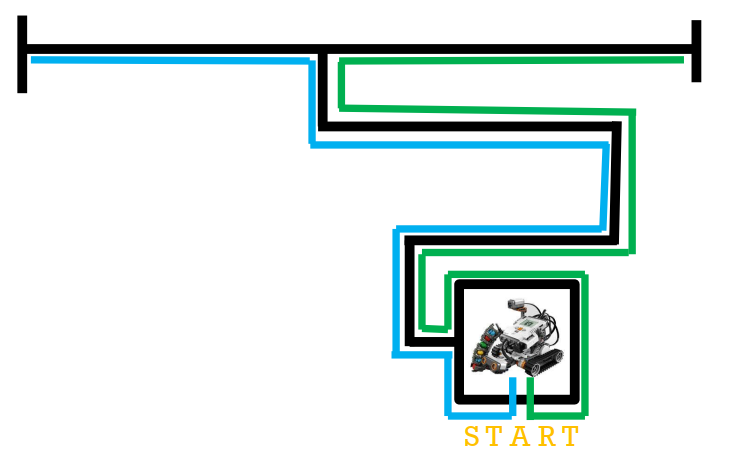
\includegraphics[scale=0.55]{figs/lineFollowingArena}
			\caption{Line following section of the race}\label{fig:lineFollowingArena.png}
		\end{figure}
		
		\begin{figure}
			\centering
			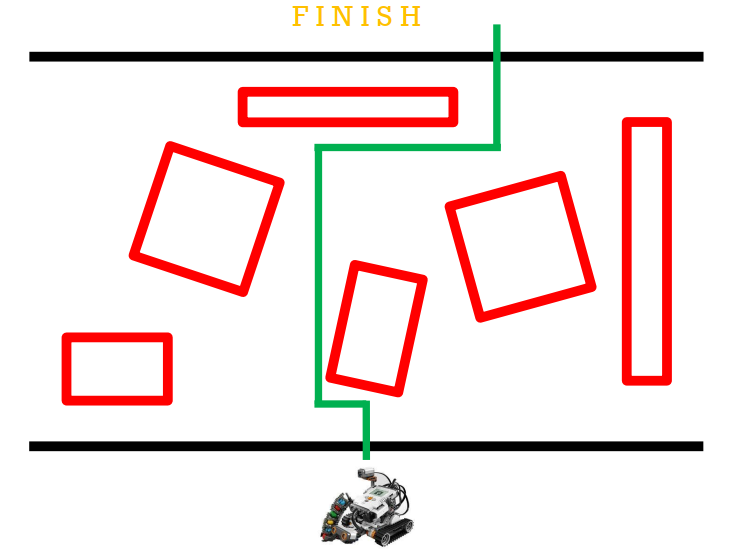
\includegraphics[scale=0.55]{figs/obstacleArena}
			\caption{Obstacle avoidance section of the race}\label{fig:obstacleArena.png}
		\end{figure}
		
		
			\section{Structure and Hardware}
			\subsection {Mechanical assembling}
			
			The mechanical assembly of the various parts and components of Arnold is shown from different perspectives in Fig. \ref{fig:arnold4trasp.png}.
			It is a classic \textit{differential drive} mobile robot whose configuration is represented by $[x,y, \theta] \in \mathbb{R}^3$.\\
			
			This structure has been designed with a castor wheel to achieve mechanical stability and proper weight distribution, and allows plenty of space to place all necessary sensors and proper cable management.\\
			Furthermore, it contains a sufficiently large gap below the brick to allow further additions (as in the case of the gyroscopic sensor) and easy battery replacement.
			
			\begin{figure}
				\centering
				\includegraphics[scale=0.15]{figs/arnold4trasp}
				\caption{Different views of the robot.}\label{fig:arnold4trasp.png}
			\end{figure}
			
			
			\subsection {Sensors}
			
			Arnold uses the following sensors:
			\begin{itemize}
				\item \textit{ \textbf {HiTechnic Gyroscope:}} measures the \textit{yaw} angular velocity as shown in Fig.\ref{fig:gyroscope.png}, so that it can be used to determine the robot orientation $\theta$ in the $\mathbb{R}^3$ configuration space, with a proper placement on the structure;
				\begin{figure}[H]
					\centering
					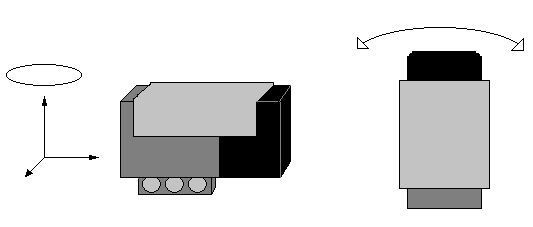
\includegraphics[scale=0.6]{figs/gyroscope}
					\caption{HiTechnic gyroscope.}\label{fig:gyroscope.png}
				\end{figure}
			
				\item \textit{\textbf {NXT Color Sensor:}} can be used to both measure RGB values of received light (unused in the project), or just the light intensity;
				
				\item \textit{\textbf {NXT Ultrasonic Sensor:}} determines the distance of an object in front of itself by emitting sound in the ultrasonic bandwidth and measuring the time between departure and reception.
				
			\end{itemize}
			
			
			
			\section{Algorithm}
			\subsection {Threading}
			
			The overall algorithm is multithreaded via the Java \textit{Thread} class, though the microcontroller used in the NXT brick (\textbf{Atmel AT91SAM7S256}) is single core, so all threads compete for the execution.\\
			
			Different threads are used for different sections of the race. Grouping them according to their purpose, they are:
			
			\begin{itemize}
				\item \textbf{Line following}
					\begin{itemize}
							\item LineFollower: implements the PID control by measuring the light intensity;
						\item SonarBumpThread: checks for the wall at the end of the line with the \textit{ultrasonic} sensor.
					\end{itemize}
				
				\item \textbf{Arenas travelling}
				\begin{itemize}
						\item GyroThread: samples the \textit{gyroscopic} sensor and perform orientation odometry, which consists in a simple integration (discrete sum) as the reconstruction of the robot angle $/theta$ from the \textit{yaw} speed is exact;
					\item ArenaTraveler: goes from line following arena to obstacle avoidance, by implementing a proportional control with respect to the angle measured by the gyroscope, while checking the starting line.
				\end{itemize}
			
				
				\item \textbf{Obstacle Avoidance}
				\begin{itemize}
					\item GyroThread: same as previous one;
					\item SonarThread: constantly rotates the ultrasonic sensor between fixed angles with an auxiliary motor while calculating distance of objects (if any) at those angles;
					\item Roamer: controls the driving motors accordingly to the orientation (used for the \textit{attractive potential}) and the distances to objects at different angles (used for the \textit{repulsive potential}).
				\end{itemize}
				
			\end{itemize}
			\vspace{7mm}
			
			For each change between sections, the relevant threads are properly exited and collected by the Java garbage collector, with the exception of the gyroscope thread between sections \RNum{2} and \RNum{3}.\\
			
			While this has allowed an easier management of the code and a more performant algorithm, it did pose some issues, mainly related to the unclear functions for thread management implemented in \textit{LeJos}: methods like
			\begin{lstlisting}
			%%Thread%%.sleep(int ms);
			\end{lstlisting}
			often don't work as expected, which results in two issues:
			\begin{itemize}
				\item trying to sleep inside the gyroscope thread for 1 ms (which is the minimum allowed) often results in sleeping for more;
				\item the \textit{Delay} class methods, which are based on \textit{Thread.sleep}, don't interrupt the calling thread as they should:
					\begin{itemize}
					\item in higher priority threads this won't result in preemption and thus lower priority ones will never execute
					\item while reading distances with 
					\begin{lstlisting}
					%%UltrasonicSensor%%.getDistance();
					\end{lstlisting}
					\emph{all} execution is blocked, as the thread isn't properly preempted, which gives significant drift in orientation odometry and delays in the PID controller for line following, of which the initial (very performing) speed had to be reduced.
				\end{itemize}
					
			
			\end{itemize}
			
			
			\subsection {Line Following}
			
			The Line Following part is performed by a PID controller on the light level and a intermittent monitoring of distance from the wall. It can be broken down into 4 parts:
			\begin{enumerate}
				\item calibration of maximum and minimum light values;
				\item escape from the square: this is simply done by commanding the robot to go forward until a value of light corresponding to the tape is seen, and to the darker floor subsequently. Once this is verified, start the line following algorithm;
				\item follow the line;
				\item stop at the wall: the ultrasonic sensor thread is activated every 350ms and checks for the wall ahead (when the distance returned is below 35cm). The length of this period is not ininfluent and a too large value may cause the robot to miss the detection and subsequent collision; however, if this period is too little, because of the reasons stated above about threading in \textit{LeJos} the PID controller would significantly lose performance because of all the non preemptable interruptions.
			\end{enumerate} 
		
			\subsection{PID control}
			The light value is read by the respective sensor and can be a value between 0 and 1023.
			The system is initialized by taking the average (over 20 samples) of both values returned when over the dark area and the light tape, which respectively compose the calibration values \emph{minLight} and \emph{maxLight}.\\
			Then, an error range is defined (in our case, 150); the error takes any value between $-range/2$ and $range/2$, in a linear fashion with respect to the actual light value, i.e. $$e=m\cdot \mathit{light}+c$$, where $$m=\mathit{range}/(\mathit{maxLight-minLight})$$, and $$c=\mathit{range}/2-m\cdot \mathit{maxlight}$$\\
			In this way, the error is equal to 0 approx. where the boundary between tape and floor lies, and any controller trying to push it to 0 will force the robot to stay on that boundary (Fig.\ref{fig:lightError.png}).\\
			\begin{figure} [H]
				\centering
				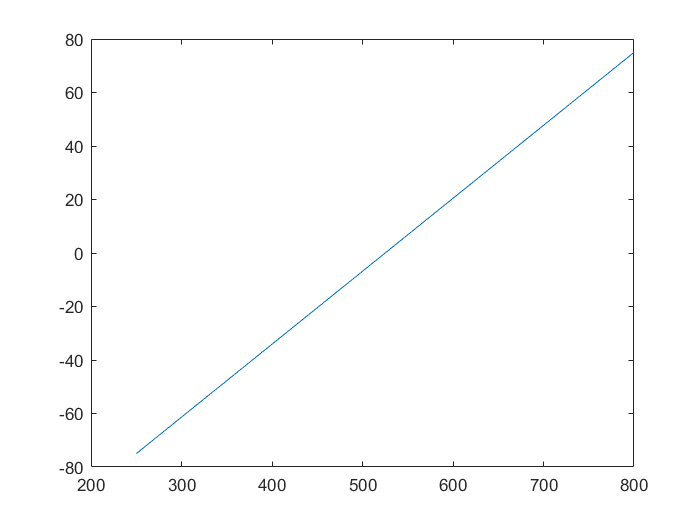
\includegraphics[scale=0.45]{figs/lightError.png}
				\caption{Light values from a minimum of 250 and a maximum of 800, with an error range of 150.}\label{fig:lightError.png}
			\end{figure}
			
			The controller is a classical PID one, acting directly on the power of the wheels, with a feedforward action on them to make the robot move forward (Fig. \ref{fig:PID_fig.png}).
			\begin{figure} [H]
				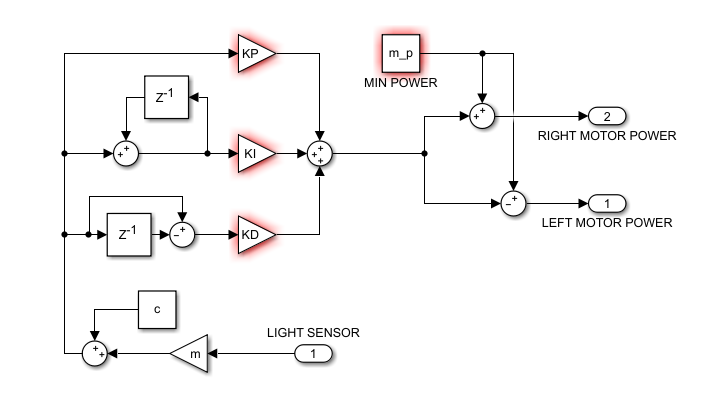
\includegraphics{figs/PID_fig.png}
				\caption{Simulink scheme of the robot controller.}\label{fig:PID_fig.png}
			\end{figure}
			
			The derivative action is simply done by multiplying the difference between the previous error and the current one; likewise, the integral gain acts on the continuous sum of the errors.\\
	
			% put here how we calibrated PID
			
			
			
			
			\subsection {Obstacle Avoidance}
			
			The obstacle avoidance algorithm is an attempt to port the \textbf{\emph{Potential Fields}} approach to a very constrained scenario.\\
			The basic idea is to define an attractive potential represented by the difference between the current measured $\theta$ of the robot and the target angle being $\pi/2$, that is the direction to go in order to traverse the arena, if considering  $\theta=0$ when we first stop the PID in front of the wall. The angle is measured by the already mentioned gyroscopic sensor.\\
			Additionally, a repulsive potential is defined by taking into considerations possible obstacle on the course ahead, their distance and angle with respect to the robot.\\
			
			However, the original formulation of this approach involve the computation of the exact \emph{gradient} at each instant, of the quantities represented by the surrounding environment. While the drifting problem of orientation odometry is not strictly related to this issue, the calculation of the obstacle distances and position is: in fact, not only the ultrasonic sensor is quite slow, but also it can just get the distance of object ahead of itself, and not around.\\
			For this reason we mounted it on a third motor, which switches between different angles, thus trying to mimic a continuous monitoring of the environment, as shown in the animation below.
			
		
			\begin{center}	
				\animategraphics[controls, scale=0.5, label=fig:sonarVisual]{15}{figs/sonarDemo/testAnimated}{0}{100}
			\end{center}
		
			
			For each sector we apply a repulsive action inversely proportional to the obstacles distance measured in that sector, while the attractive function tries to maintain the robot along the direction parallel to the walls ($\pi/2$). By neglecting all the distances greater than a certain threshold, along relatively free space sections the robot should proceed along a straight line. Ideally, the control should be:
			
				$$u_{left} = minPower + \nabla U$$
			    $$u_{right}= minPower + \nabla U$$
			    
			with:
			
				$$U = U_{att} + U_{rep} $$
				
			However, due to the issue mentioned previously, we can just approximate $U_{rep}$,
				
				
				
				
				
				
			
			\section{Performances}
			
			
			
			
			
			
			%%%%%%%%% CAPITOLO  %%%%%%%%%%%%%%%%
			\chapter{Matlab Simulations}
			
			\section{Section title}
			\subsection {Subsection title}
			
			
			
			%%%%%%%%%%%%%%%%%%%%%%%%%%%%%%%%%%%%%
			
			
			
			% %%%% APPENDIX %%%%%
			% \appendix
			% \chapter{Appendix title}
			% %%%%%%%%%%%%%%%%%%%%
			
			%%%%%%%%%% BIBLIOGRAPHY %%%%%%%%%%%%%%
			\bibliography{bibliography}{}
			\bibliographystyle{plain}
			\addcontentsline{toc}{chapter}{Bibliography}
			%%%%%%%%%%%%%%%%%%%%%%%%%%%%%%%%%%%%%%
			
			\end{document}